\chapter{Algebra and Functions: Part II}

\headertitle{Graphs of Parent Functions}

\medskip
Often times knowing what the general graphs of functions will give you insight into a problem, like solving for the intercepts of a linear function, or the minimum of a quadratic function. The graphs of the most common functions are listed below:

\bigskip
\begin{figure}[h]
\pgfplotsset{ticks=none}
\centering
\begin{minipage}[b]{0.45\linewidth}
\centering
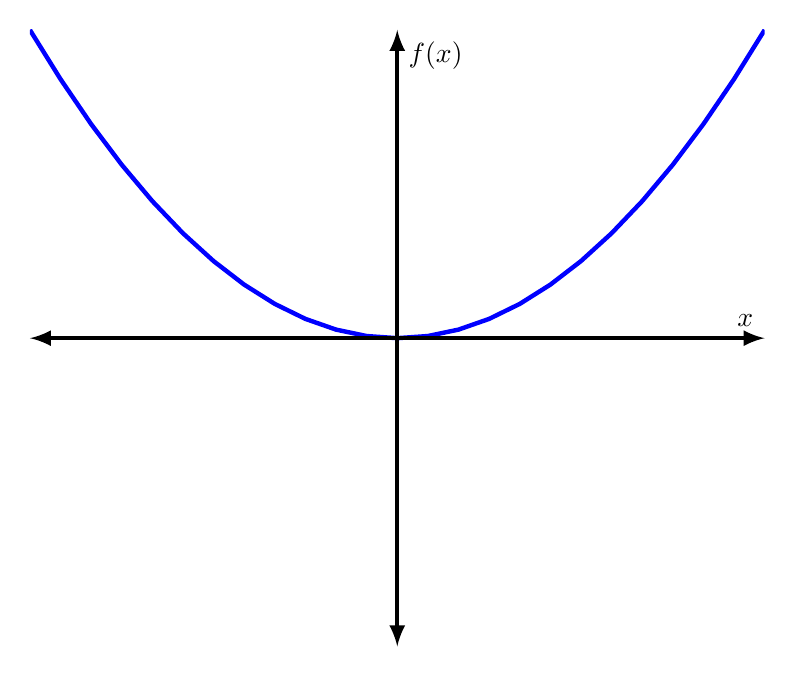
\begin{tikzpicture}[scale=1]
\begin{axis}[axis x line=middle, axis y line=middle, ymin=-25, ymax=25, ylabel=$f(x)$, xlabel=$x$, ultra thick, axis line style=latex-latex, axis on top=true, width=0.9\textwidth]
\addplot[domain=-5:5, blue, ultra thick] {x^2};
\end{axis}
\end{tikzpicture}
\caption{$f(x)=x^2$}
\label{fig:subfigure1}
\end{minipage}
\quad
\begin{minipage}[b]{0.45\linewidth}
\centering
\begin{tikzpicture}[scale=1]
\begin{axis}[axis x line=middle, axis y line=middle, ymin=-10, ymax=10, xmin=-10, ylabel=$f(x)$, xlabel=$x$, ultra thick, axis line style=latex-latex, axis on top=true, width=0.9\textwidth]
\addplot[domain=0:10, blue, ultra thick] {sqrt(x)};
\end{axis}
\end{tikzpicture}
\label{fig:subfigure2}
\caption{$f(x)=\sqrt{x}$}
\end{minipage}

\bigskip
\begin{minipage}[b]{0.45\linewidth}
\centering
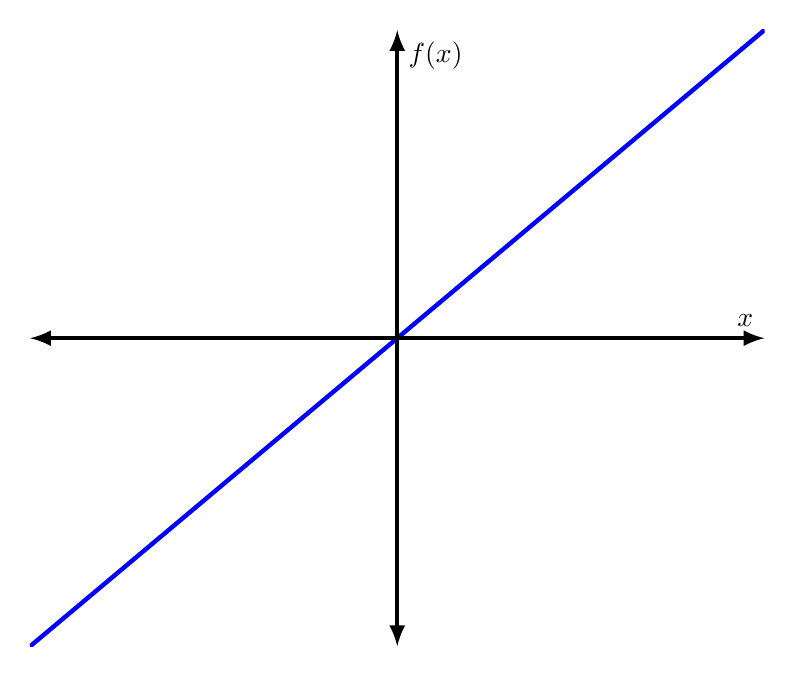
\begin{tikzpicture}[scale=1]
\begin{axis}[axis x line=middle, axis y line=middle, ymin=-10, ymax=10, xmin=-10, ylabel=$f(x)$, xlabel=$x$, ultra thick, axis line style=latex-latex, axis on top=true, width=0.9\textwidth]
\addplot[domain=-10:10, blue, ultra thick] {x};
\end{axis}
\end{tikzpicture}
\caption{$f(x)=x$}
\label{fig:subfigure3}
\end{minipage}
\quad
\begin{minipage}[b]{0.45\linewidth}
\centering
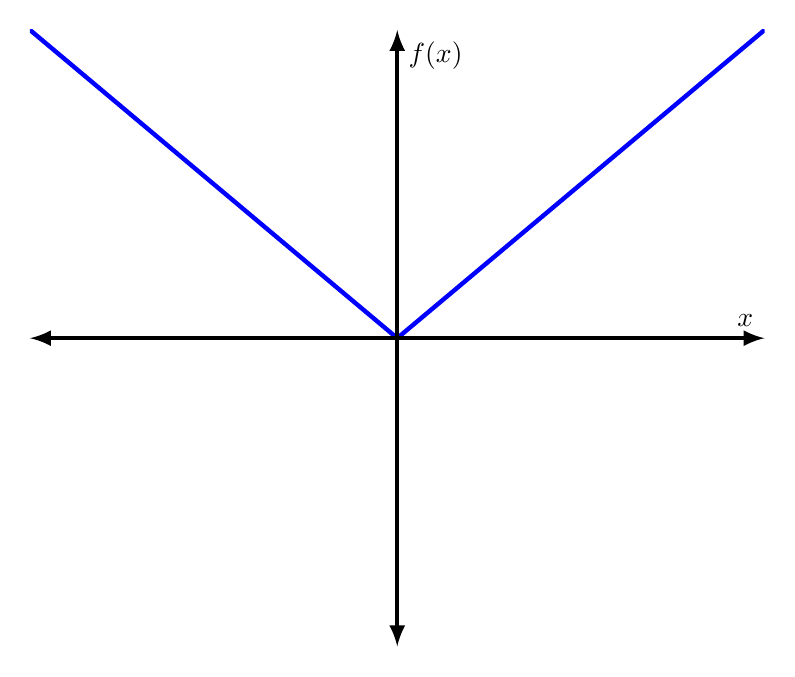
\begin{tikzpicture}[scale=1]
\begin{axis}[axis x line=middle, axis y line=middle, ymin=-10, ymax=10, xmin=-10, ylabel=$f(x)$, xlabel=$x$, ultra thick, axis line style=latex-latex, axis on top=true, width=0.9\textwidth]
\addplot[domain=-10:10, blue, ultra thick] {abs(x)};
\end{axis}
\end{tikzpicture}
\caption{$f(x)=|x|$}
\label{fig:subfigure4}
\end{minipage}
\end{figure}